\documentclass[a4paper,16pt]{article}
\usepackage[left=2cm,right=2cm,
top=2cm,bottom=2cm,bindingoffset=0cm]{geometry}
\usepackage{cmap}
\usepackage[T2A]{fontenc}
\usepackage{amsmath,amssymb,amsfonts,amsthm,mathtools}
\usepackage[utf8]{inputenc}
\usepackage{fancybox,fancyhdr}
\usepackage{euscript,mathrsfs}
\DeclareMathOperator{\tg}{tg}
\DeclareMathOperator{\I}{I}
\DeclareMathOperator{\II}{II}
\DeclareMathOperator{\III}{III}

\usepackage[english]{babel}
\usepackage{icomma}


\fancyhead[R]{Якимов Г.В.}
\fancyhead[L]{}
\fancyhead[C]{}

\fancyfoot[R]{}
\fancyfoot[L]{}
\fancyfoot[C]{}

\begin{document}
	\pagestyle{fancy}
	\graphicspath{{figures/}}

	\title{Расчетное задание}
	\author{Якимов Г.В., гр. 19122}
	\maketitle

	Выборка: 25


	1. $\overrightarrow{X} \sim N(a, \sigma^2)$

	a)

	\begin{center}
	$$\I. \ G(\overrightarrow{X}, a) = \sqrt{n} \cdot \dfrac{\overline{X} - a}{\sigma} \sim N(0, 1)$$
	$$\II. \ t: P\biggr(-t < \sqrt{n} \cdot \dfrac{\overline{X} - a}{\sigma} < t\biggr) = 1 - \varepsilon \Rightarrow t = \tau_{1-\varepsilon/2}$$
	$$\III. \ P\biggr(\overline{X} -  \tau_{1-\varepsilon/2} \cdot \frac{\sigma}{\sqrt{n}} < a < \overline{X} + \tau_{1-\varepsilon/2} \cdot \frac{\sigma}{\sqrt{n}}\biggr) = 1 - \varepsilon$$
	\end{center}
	Ответ: $\overline{X} = ; \ \tau_{1-\varepsilon/2} = ; \ P\biggr( < a < \biggr) = 0.95$

	б)

	\begin{center}
	$$\I. \ G(\overrightarrow{X}, a) = \sqrt{n} \cdot \dfrac{\overline{X} - a}{S_0^2} \sim N(0, 1)$$
	$$\II. \ t: P\biggr(-t < \sqrt{n} \cdot \dfrac{\overline{X} - a}{S_0^2} < t\biggr) = 1 - \varepsilon \Rightarrow t = \tau_{1-\varepsilon/2}$$
	$$\III. \ P\biggr(\overline{X} -  \tau_{1-\varepsilon/2} \cdot \frac{S_0^2}{\sqrt{n}} < a < \overline{X} + \tau_{1-\varepsilon/2} \cdot \frac{S_0^2}{\sqrt{n}}\biggr) = 1 - \varepsilon$$
	\end{center}
	Ответ: $S_0^2 = ; \ P\biggr( < a < \biggr) = 0.95$

	в)

	\begin{center}
	$$\I. \ G(\overrightarrow{X}, a) = \sqrt{n} \cdot \dfrac{\overline{X} - a}{\sigma} \sim N(0, 1)$$
	$$\II. \ t: P\biggr(-t < \sqrt{n} \cdot \dfrac{\overline{X} - a}{\sigma} < t\biggr) = 1 - \varepsilon \Rightarrow t = \tau_{1-\varepsilon/2}$$
	$$\III. \ P\biggr(\overline{X} -  \tau_{1-\varepsilon/2} \cdot \frac{\sigma}{\sqrt{n}} < a < \overline{X} + \tau_{1-\varepsilon/2} \cdot \frac{\sigma}{\sqrt{n}}\biggr) = 1 - \varepsilon$$
	\end{center}
	Ответ: $\overline{X} = ; \ \tau_{1-\varepsilon/2} = ; \ P\biggr( < a < \biggr) = 0.95$

	г)

	\begin{center}
	$$\I. \ G(\overrightarrow{X}, a) = \sqrt{n} \cdot \dfrac{\overline{X} - a}{\sigma} \sim N(0, 1)$$
	$$\II. \ t: P\biggr(-t < \sqrt{n} \cdot \dfrac{\overline{X} - a}{\sigma} < t\biggr) = 1 - \varepsilon \Rightarrow t = \tau_{1-\varepsilon/2}$$
	$$\III. \ P\biggr(\overline{X} -  \tau_{1-\varepsilon/2} \cdot \frac{\sigma}{\sqrt{n}} < a < \overline{X} + \tau_{1-\varepsilon/2} \cdot \frac{\sigma}{\sqrt{n}}\biggr) = 1 - \varepsilon$$
	\end{center}
	Ответ: $\overline{X} = ; \ \tau_{1-\varepsilon/2} = ; \ P\biggr( < a < \biggr) = 0.95$


	2.

	3. 
	\begin{figure}[h]
		\center{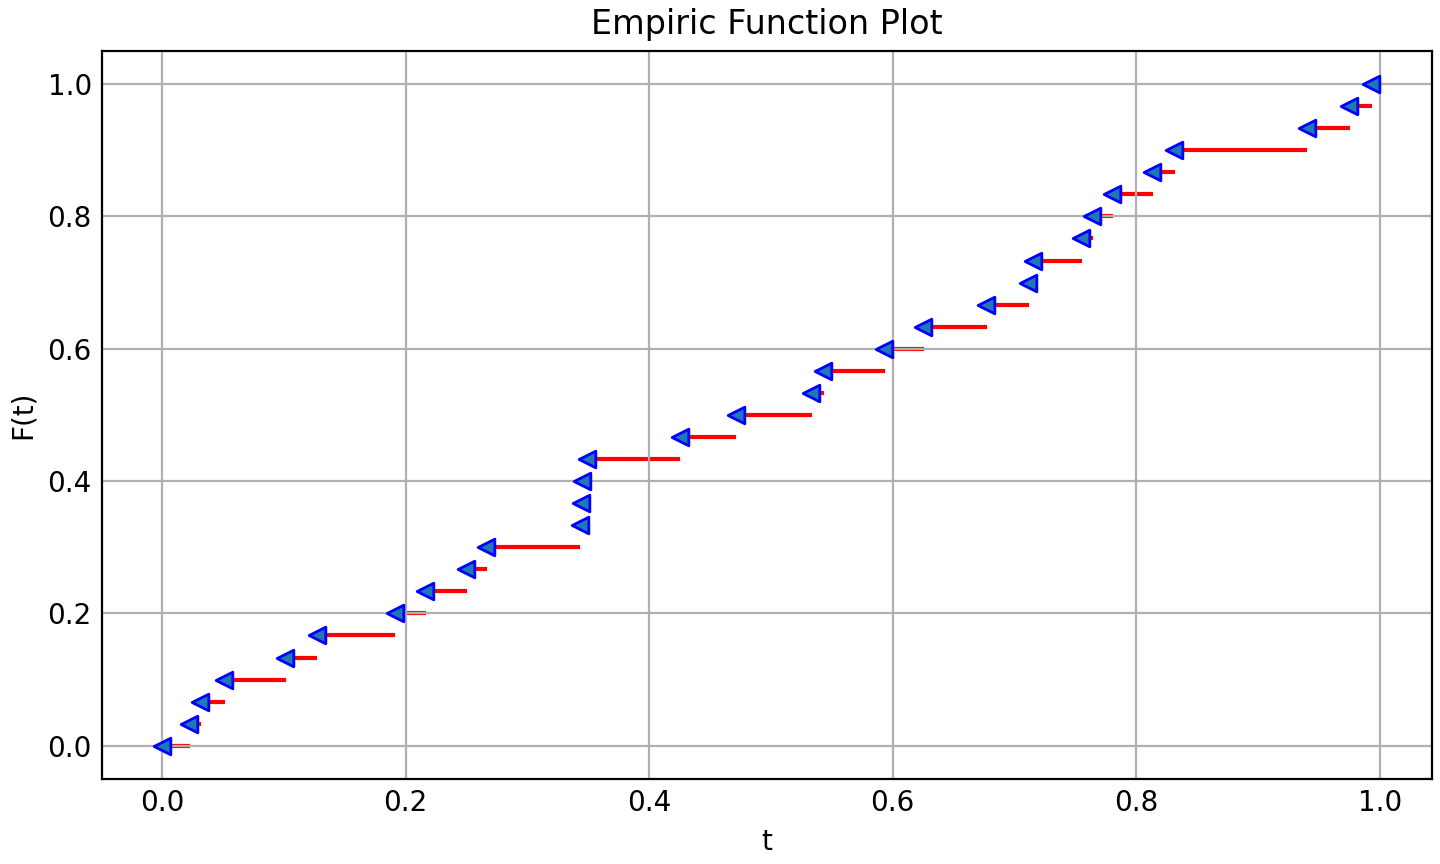
\includegraphics[scale=0.9]{Figure_1.png}}
		\caption{График эмпирической функции распределения}
		\label{fig:image}
	\end{figure}
	\end{document}